\chapter{Simulation}
\label{sec:simulation}
In this chapter I discuss how high energy particle
collisions are simulated. Simulated collisions, based on knowledge of the standard model, provide 
the foundation of our predictions in high energy particle physics. 
The wealth of particle physics knowledge accumulated over the last 
60 years has provided a testing grounds to compare experimental results with
simulated particle collisions. Based on past experiments and extensive work from the simulation community,
we are able to simulate and model the the proton-proton collisions which take place in the
CMS detector with a high degree of precision. 
In this thesis, we are specifically interested in comparing two physics scenarios: the standard model 
without the existence of a 125\GeV Higgs boson versus the standard model with the existence
of a 125\GeV Higgs boson. Both of these predictions rely on the standard model processes and
Higgs boson processes being well modeled via simulation.
In the following sections, I briefly discuss how events are simulated for proton-proton collisions,
how the initial products of the collision decay, the steps of parton showering,
fragmentation and hadronization, and how the decay products are simulated
to interact with a model of the CMS detector.

There are many different Monte Carlo (MC) event generators which can contribute to the 
simulation of high energy particle collisions and decays. There are three main MC event
generators which are commonly used to model the full proton-proton collision: 
\PYTHIA~\cite{Sjostrand:2014zea}, \HERWIG~\cite{Bahr:2008pv}, and \textsc{Sherpa}~\cite{Gleisberg:2008ta}
including both hard scattering processes and subsequent evolution of the products to final 
state products. Several other generators, including \POWHEG~\cite{Alioli:2010xd,Frixione:2007vw}
and \MGAMCNLO~\cite{Alwall:2011uj,Alwall:2014hca}, 
are also used to model only hard scattering processes and, in this thesis, 
interface to \textsc{Pythia8}~\cite{Sjostrand:2014zea} for evolution to the final state products.
\textsc{Pythia8} includes a set of physics models
which can simulate the particle evolution from a few-body hard-scattering process through
to a complex multiparticle final states.

To produce the physics processes used in this
thesis we rely on MC event generators besides \textsc{Pythia8} for the hard-scattering process.
Then we switch back to \textsc{Pythia8} to evolve the hard-scatter products through 
to their final state products. The
choice to stitch together multiple MC generators is made when the internal
hard-scattering physics library in \textsc{Pythia8} is not as complete as other generators or other
generators are able to achieve higher order accuracy in their treatment of the
hard-scattering process.

The signal samples with a Higgs boson produced through gluon fusion ($\cPg\cPg\PH$), vector boson fusion (VBF),
or in association with a $\PW$ or $\PZ$ boson ($\PW\PH$ or $\PZ\PH$), are all
generated at next-to-leading order (NLO) in perturbative quantum chromodynamics~\cite{REYA1981195} 
with the \POWHEG 2.0~\cite{Nason:2004rx,Frixione:2007vw, Alioli:2010xa, Alioli:2008tz} 
generator. Details on these four Higgs boson processes can be found in the Higgs Phenomenology chapter
Section~\ref{sec:higgs_production} and Figure~\ref{fig:higgs_feyn}. 
The \textsc{minlo hvJ} extension of \POWHEG 2.0 
is used for the $\PW\PH$ and $\PZ\PH$ simulated samples~\cite{Luisoni:2013kna}. 
%The $\ttbar\PH$ process has a is negligible.
The \POWHEG 2.0 generator is used for the $\ttbar$, $\Pq\Pq \to \PZ\PZ$, and $\PW\PZ$
standard background processes while \POWHEG 1.0 is used for simulating 
single top quark production.
Additionally, \POWHEG is used for the $\PW\PH \to \PW\PW\PW$, $\PZ\PH \to \PZ\PW\PW$,
and $\hzz$ backgrounds which all include non-signal Higgs bosons production and decay.
The \MGAMCNLO generator is used for the $\PZ+$jets, $\PW+$jets, $\ttbar \PZ$, and triboson
processes to simulate events at leading order (LO)~\cite{Alwall:2007fs}.
The \MGAMCNLO generator is used for diboson and $\ttbar \PW$ production simulated at next-to-LO (NLO) 
%with the FxFx jet matching and merging
~\cite{Frederix:2012ps}.
The $\Pg\Pg \to \PZ\PZ$ process is generated at leading order (LO) with 
\textsc{MCFM}~\cite{Campbell:2010ff}. 



\section{Hard-Scattering Process}
The hard-scattering process is the main process of interest in a simulated event.
It is the portion of the simulation describing the interaction and annihilation of the
two partons from the colliding protons. The hard-scattering process creates the 
signal and background processes of interest in this thesis,
such as $\PW$, $\PZ$, and Higgs bosons. For all simulated signal and background samples,
the hard-scattering process is defined by the standard model Lagrangian. The specific processes
studied in this thesis can be represented by matrix elements and their
resulting Feynman diagrams.

The \MGAMCNLO generator can be
operated at both LO and NLO accuracies. After supplying \MGAMCNLO with a process of interest including
the input partons and resulting particles, it generates the Feynman rules describing the 
process and can translate them into Feynman diagrams~\cite{Christensen:2008py}. 
At LO, this process is fully automated using \textsc{FeynRules}~\cite{Christensen:2008py,Alloul:2013bka}.
At NLO, the NLO QCD, the process is fully automated via \textsc{FeynRules}; other NLO contributions 
%such as UV counter-terms 
must be added with dedicated computations~\cite{Alwall:2014hca}.

The \POWHEG event generator is used for production of the Higgs boson signal processes in
this thesis. \POWHEG does not have the convenient automation which comes with \MGAMCNLO, instead each
physics process must be coded separately. However, the large amount of interest in Higgs boson physics
has led to a thoroughly developed and validated process library resulting in NLO accuracy
~\cite{Alioli:2010xa,Alioli:2008tz,Brein:2003wg,Ravindran:2003um,deFlorian:2012mx}.
%Additionally, \POWHEG is used for the Higgs signal process because it often produces a more 
%reliable $\pt$ spectrum and more accurate description of the hard jets~\cite{Frixione:2007vw,Alioli:2010xd}.




\section{Parton Distribution Functions}
\label{sec:sim_pdf}
One of the unique complexities present at a hadron collider, which is avoided with a
lepton collider, is accounting for the substructure of the colliding hadrons. 
We must account for this to create proper simulations
of LHC proton-proton collisions. The internal structure of the proton
has been probed over the past half century through deep inelastic scattering
experiments~\cite{Breidenbach:1969kd, PhysRevLett.23.930}.
Experimental results show the internal structure of protons revealing the existence of
quarks and gluons. It is these quarks and gluons which collide and interact in
proton-proton collisions.
The probability for each quark or gluon to have a certain fraction
of the proton's momentum is given by the parton distribution function (PDF).
The PDFs depend on the energy scale of the proton. All simulations
in this thesis rely on PDFs for an energy scale of 6.5\TeV matching the LHC beam.
%Figure~\ref{fig:sim_pdf} 
%shows example PDFs for two given energy scales. 

The specific PDFs which are used in this thesis
 are provided by \texttt{NNPDF3.0} with the exact PDF set being 
\texttt{NNPDF30\_nlo\_as\_0118}~\cite{Ball:2014uwa, Ball:2011uy}. The \texttt{NNPDF3.0} PDFs
are derived using a global dataset including, but not limited to, data from HERA, ZEUS, ATLAS, LHCb, and CMS.
Functional forms derived from theoretical QCD predictions with electroweak corrections are fit
to the available data~\cite{Ball:2014uwa}.
The PDFs provide proper normalization based on the probabilistic distribution of the 
available partons and their energies as inputs to the hard-scattering process.
%Uncertainties from the PDF estimation method are applied in the following analyses to cover
%potential mismodeling of the proton PDFs used in the CMS simulations.



\section{Underlying Event}
In addition to the particles resulting from the hard-scattering portion of a proton-proton collision,
there are additional particles resulting from what is called the underlying event. 
The underlying event consists of interactions between
partons which are not directly associated with hard-scattering event, for example secondary partons 
within the colliding protons.
Underlying event collisions are softer and lower energy in nature which limits the range of 
the resulting physics processes. 
The most common underlying event interactions result in two partons interacting resulting in a 
single parton which then combines with other partons to form outgoing hadrons. 
This is only an intermediary stage as color confinement eliminates the possibility
of a single isolated parton propagating through the CMS detector, this will be revisited shortly.

The underlying event in 
Monte Carlo event generators characterize the kinematics and composition of soft ``jets''.
There are specific ``jet'' related physics observables which are sensitive to the characteristics of the underlying
event~\cite{Khachatryan:2015pea, Field:cdf2008}. For a description of ``jets'' see Section~\ref{sec:obj_reco_jets}.
The initial underlying event tune for \textsc{Pythia8} is the Monash Tune~\cite{Skands:2014pea}. 
A CMS specific tuning of 
\textsc{Pythia8} has been constructed based off of the parameters of the Monash Tune but adding 
some additional energy-dependent parameters to the fit. The tune is based
on data from CDF and 7 \TeV CMS data and is called \texttt{CUETP8M1}.
Considering \texttt{CUETP8M1} is derived based largely on data from
CMS, there is very good agreement between CMS data and simulations based on the
\texttt{CUETP8M1} tune~\cite{Khachatryan:2015pea}. 



\section{Parton Showers}
While matrix elements are used to calculate the hard-scattering event, 
the use of matrix elements to fully describe the production and decay of all of the
partons is technically not possible with current best Monte Carlo generators~\cite{PhysRevD.94.074005}. 
Instead, parton shower programs handle radiation of soft gluons from 
color charged particles and photons from electrically charged particles~\cite{Sjostrand2005}.
Initial state radiation (ISR) occures when an incoming charged particle radiates before entering the 
hard-scattering process~\cite{PDG}. When an outgoing particle radiates, it is called
final state radiation (FSR).
Partons from ISR, FSR, the underlying event and the hard-scatter 
process are decayed using the parton shower method. 

Parton shower evolution can be viewed as a probabilistic process 
where each produced parton has a probability
of radiating another parton. Partons iteratively emit other partons through three 
dominant processes: $\textrm{q} \to \textrm{gq}$, $\textrm{g} \to \textrm{gg}$, 
and $\textrm{g} \to \textrm{q}\bar{\textrm{q}}$. Swap $\textrm{q}$ for $\bar{\textrm{q}}$
to complete the set. 

Technically, there is a matching and merging of the hard-scatter matrix element with the
parton shower contribution. This does not affect the total process cross section.
The $\PZ+$jets and $\PW+$jets samples, which were simulated with \MGAMCNLO at LO, 
use MLM jet matching and merging~\cite{Alwall:2007fs}.
The diboson production samples simulated with \MGAMCNLO at NLO use the 
FxFx jet matching and merging~\cite{Frederix:2012ps}. 
In contrast, \POWHEG 2.0 and 1.0 are used for \ttbar
The Monte Carlo generators used in this thesis are interfaced with 
\PYTHIA 8.212~\cite{Sjostrand:2014zea} to model the parton shower evolution.



\section{Fragmentation and Hadronization}
As mentioned previously, due to color confinement, quarks and gluons cannot exist in isolation
and must be transformed in color-neutral final states~\cite{Hoche:2014rga}. 
To resolve the lone quarks and gluons which resulted from the hard-scatter process and the parton 
shower, the partons undergo hadronization. Hadronization is the process where hadrons are formed 
out of quarks and gluons. There are multiple phenomenological models of hadronization, the
specific one used in this thesis is the Lund String Model~\cite{Sjostrand:1985ys}. 
The Lund String Model of jet
hadronization is based the observation that within a meson system the quark-antiquark 
potential rises linearly with the distance between quarks~\cite{Bali:1992ab}. In the model, this
potential energy is stored in flux lines connecting the quark-antiquark pair, see left pane 
Figure~\ref{fig:sim_lund_string}. As a quark-antiquark 
pair with high energy moves apart the energy stored between them in the flux lines increases. If the energy
is sufficiently high the flux line can be severed and a second quark-antiquark pair created from
the freed energy. This can be visualized in the right pane of Figure~\ref{fig:sim_lund_string}.
This process repeats itself creating stable mesons and baryons where the low energy (anti)quarks
oscillate about each other stably, represented as the zig-zag lines in Figure~\ref{fig:sim_lund_string}.

\begin{figure*}[htbp]
\centering
     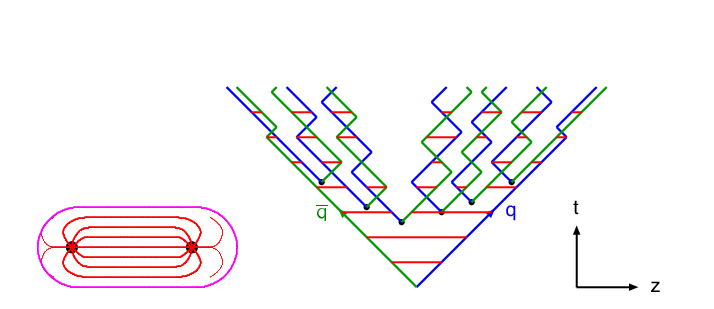
\includegraphics[width=0.7\textwidth]{simulation/plots/lund_time-space.png}
     \caption{
(left) Lund String Model flux tubes connecting a quark-antiquark pair. (right) A
space-time representation of the hadronization of a quark-antiquark pair. 
The final representation depicts a seven mesons final state.
     }
     \label{fig:sim_lund_string}
\end{figure*}

\textsc{Pythia8} also decays vector boson sometimes creating pairs of quarks where
it then models the subsequent parton shower, fragmentation, and hadronization.
In addition, \textsc{Pythia8} is also used to model $\tau$ lepton decays where the spin
correlations are fully included. All $\tau$ decay modes with branch ratios greater than 0.04\%
are included in the simulation~\cite{ILTEN201477}.



\section{Pileup}
\label{sec:sim_pu}
There were 27 proton-proton collisions per bunch crossing on average
in the 2016 data collected by CMS.
For most bunch crossings all of these proton-proton collisions are soft
scattering events and, with no hard process present, the event is unlikely to be stored for
future physics analysis because it will fail the Level-1 or High Level Trigger selections. 
When there is a hard-scattering process present in a bunch crossing,
the soft scattering collisions will still be present and must be modeled. 
To emulate this effect in simulated events, in addition to the two protons involved in the 
hard-scattering interaction, additional soft proton-proton collisions are added.
These collisions are referred to as ``pileup'' and are generated using
\textsc{Pythia8}. 
The distribution of the number of soft scattering events added to a simulated 
sample is intended to align with the distribution observed in the 2016 data.
Because alignment is never 100\% perfect immediately after the samples are simulated, the simulated events
are weighted to adjust their distribution to the data based on the measured instantaneous
luminosity for each bunch crossing which 
varies with time and changes through an LHC fill, see Section~\ref{sec:htt_mc_samples}.



\section{Detector Simulation}
At this stage of event simulation, the simulated events model our best approximation
of the proton-proton collisions and resulting decays and hadronization taking place
in the CMS detector. There is one critical last step to complete the event
simulations. The decay products must interact with a simulated
model of the CMS detector. The result of this final stage is simulated events that
are stored in the same data format as the data gathered by the detector itself,
raw energy deposits and tracker hits.

The \textsc{Geant4} software toolkit is used to simulate the CMS 
detector~\cite{Agostinelli:2002hh}. At its most basic, \textsc{Geant4} is a 
toolkit for simulating the passage of particles through matter. It contains a 
vast library of functionality allowing the creation of model physics detectors
made out of any desired material and in any desired geometrical configuration.
To initially validate the \textsc{Geant4} modeling of the CMS detector, test beam data and
collision data are used. Good agreement is seen between the data and the
simulated particles passing through the CMS detector for the energy response
and resolution for pions and protons~\cite{geant4_cms_2017}.

After the decay products of the simulated events have passed through the \textsc{Geant4}
simulation, they are stored in the same format as data is originally gathered. From
this point forward, data and simulated events are reconstructed with the exact same 
algorithms.




